% Allow relative paths in included subfiles that are compiled separately
% See https://tex.stackexchange.com/questions/153312/
\providecommand{\main}{..}
\documentclass[\main/thesis.tex]{subfiles}

\onlyinsubfile{\zexternaldocument*{\main/tex/introduction}}

\begin{document}

\chapter{Novel Generations}

\label{gens}
\section{The Pipeline}
 With our \emph{synth generator} and \emph{virtual ear} in place we can quickly generate random virtual synthesizer programs. Once we render the virtual synthesizers with these programs and create the corresponding audio sample, we can categorize the audio sample. Simply put, we randomly create drum programs and generate and the corresponding signal. This signal is then fed through $Phase 1$ and $Phase 2$ of our ear model to determine if the signal is percussive. If so, a category is assigned to our sound. This sound can then be saved as an audio file, and its virtual synthesizer can also be saved.
 
 With our current model, a single iteration of this pipeline will take approximately 50 milliseconds for Synthesizers with stack sizes of 8 or less. This means around 20 iterations can be done per second using a single process. This pipeline scales up efficiently with multiprocessing. We have not measured the iteration latency for this pipeline when a GPU is leveraged. For reference, our CPU measurements are collected on a 2012 Macbook Air running Ubuntu 18.04.
 In future work we will attempt guided generation via genetic and other heuristic search methods. Here we attempt a deep analysis of the randomly generated samples and the corresponding scores given by the ear. This analysis can expose weaknesses in our methodology which can be improved for future works where various search methods will be evaluated.
  


 \section{Survey of Two-Phased Ear Performance}
\label{survey:2p}
\begin{figure}[H]
    \begin{center}
    \makebox[\textwidth]{
    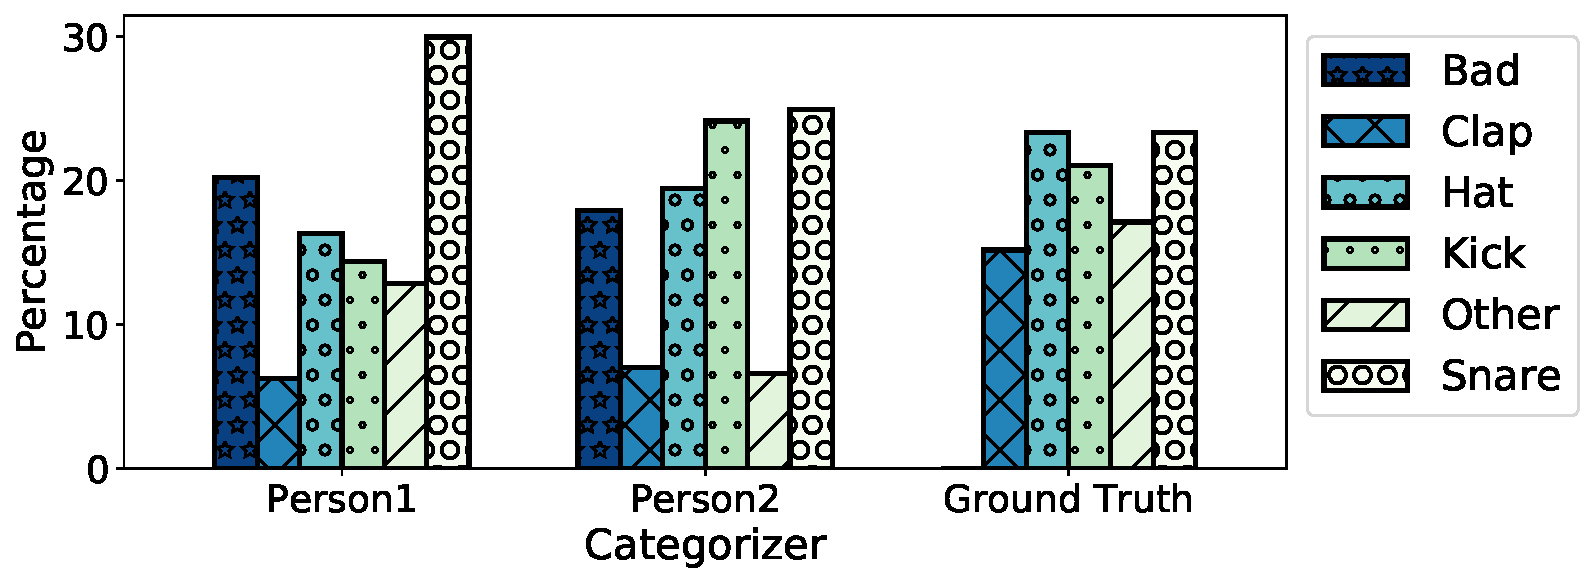
\includegraphics[width=1.1\linewidth]{images/chapter_4/cat_2p.pdf}}
    \end{center}
    \caption{Frequency of assigned labels for the categorizations by persons and the average categorizer}
\label{fig:freq-survey-2p}
\end{figure}
To measure the quality of the samples produced by our pipeline and the power of our models, we randomly generated around 50-60 samples in the following categories: "snare", "kick", "hat", "clap" and "other" (combination of rims, 
shakers and unusual percussive sounds"). These samples were determined to be percussive and then categorized by 4 different models (FC, CNNLSTM, E+F and AVG). We ensured a balanced division between samples of stack size 1, 2 and 4 (each stack is responsible for a third of the samples under each category). Both reviewers then categorized these samples without knowledge of other categorizations (human or computation models). It's important to note:
\begin{itemize}
    \item Humans had an additional category of "bad" for samples that they deemed not percussive. The "bad" category indicates that the sample should have been skipped in Phase 1. 
    \item With 6 categorization groups, humans had the same categorization in 47\% of cases.
    \item The agreement between the humans and AVG was 44\% and 47\%, not significantly lower than agreement with each other. 
    \item Of 257 samples humans agreed with FC, CNNLSTM, AVG and E+F respectively in 78, 76, 76 and 46 of cases.
\end{itemize}

We assess the reliability of agreement between humans and categorization models via the Fleiss' kappa coefficient \cite{fleiss1971measuring}. The value of 0 or less for this coefficient indicates no agreement beyond random chance, and the value of 1 indicating perfect agreement. Our kappa measurements \ref{kappa_table} lie within the 3.5-4.5 range, indicating mild to moderate agreement between humans and machines. We again measure this coefficient after dropping samples that were categorized as "bad" by the authors, as samples that humans deem to be "bad" indicate a failure in Phase 1 and arguably should not have been categorized by the models at all. Dropping of samples that both authors deemed "bad" causes an 8\% reduction of our data (21 samples) and a small increase in kappa score. Dropping samples deemed bad by either reviewer resulted in a 30\% reduction of samples and relatively large increase in kappa scores. 
Possible takeaways from this survey:
\begin{itemize}
    \item The survey brings into question the reliability of our phase 1 models, as 30\% of the generated samples were deemed not percussive by at least 1 reviewer and 8\% by both reviewers
    \item The task of categorizing synthetic drums is difficult. Survey shows that the scale of agreement within humans as well as between humans and various model combinations is moderate at best, even after removal of "bad" samples.  While the same models can easily achieve 98+ percent accuracy when tested on recorded drum samples. This may be a manifestation of the "open set recognition" problem. 
    \item While there is much room for improvement, our pipeline can generate and categorize drums and percussive sounds with a promising degree of success. 
\end{itemize}
\begin{center}

\begin{table}
 \resizebox{\linewidth}{!}{\begin{tabular}{||c c c c c c c||} 
 \hline
 Drop Bad? & Size & HvH & H+FC & H+CNN & H+ALL & 3 models \\ [0.5ex] 
 \hline
 No & 257 &0.37 & 0.35 & 0.35 & 0.36 & 33\\ 
 \hline
 if both & 236 & 0.31 & 0.37 & 0.37 & 0.38 & 33 \\
 \hline
 if either& 180 & 0.47 & 0.50 & 0.48 & 0.46 &  0.37 \\
 \hline
\end{tabular}}
\caption{\label{kappa_table}Table of Fleiss' kappa coefficient to measure the degree of agreement between humans (HvH), humans with FC model (H+FC), humans with CNNLSTM model, humans with all models (H+ALL), and the 3 models }
\end{table}
\end{center}

 \section{Survey of Two-Phased Ear Performance}
\label{survey:2p}
\begin{figure}[H]
    \begin{center}
    \makebox[\textwidth]{
    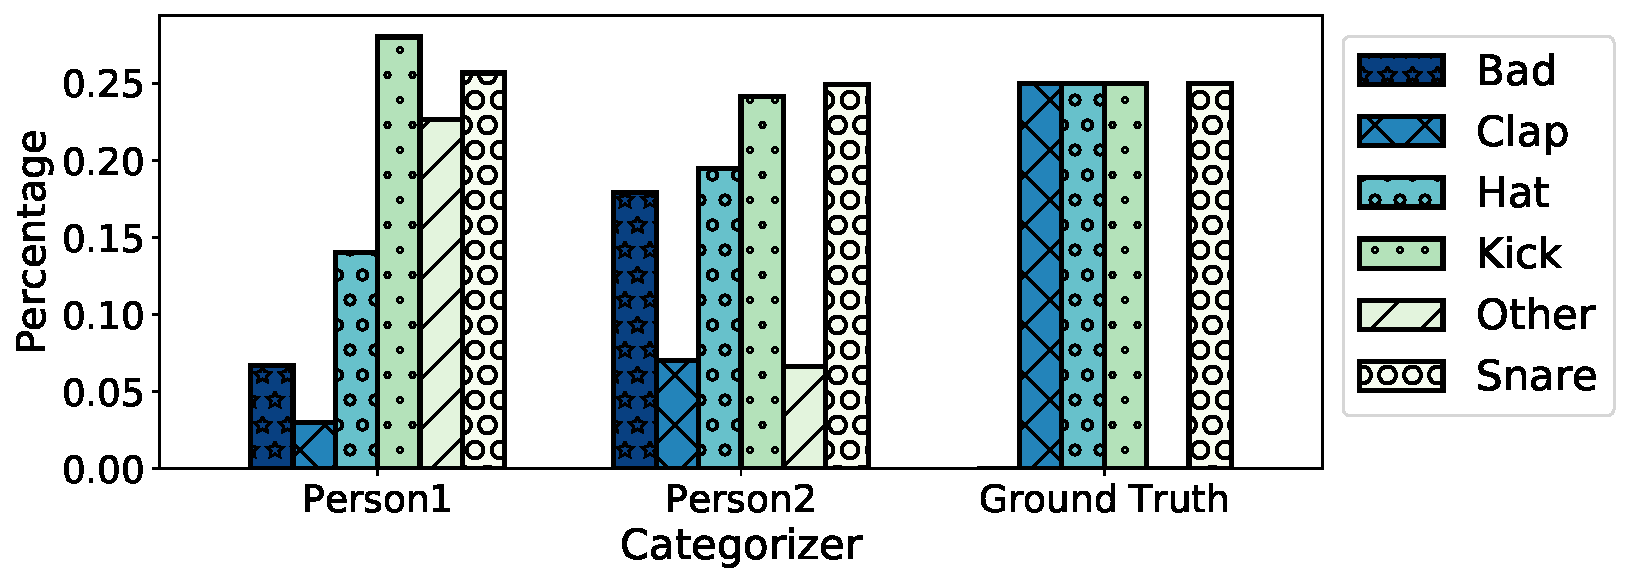
\includegraphics[width=1.1\linewidth]{images/chapter_4/cat_mme.pdf}}
    \end{center}
    \caption{Frequency of assigned labels for the categorizations by persons and the Mixed Ear Model}
\label{fig:freq-survey-2p}
\end{figure}
\section{Genetic Search}
%  introduce genetic search and how it works for our project
% 3 graphs for 3 stack sizes trying to find a certain type of drum

\end{document}